\section[Фигура 1]{Фигура 1}
Используя инструмент \textbf{\textit{Bezierline}}, строим кривую.
Копируем полученную кривую, перемещаем по горизонтали.
Применяем инструмент \textbf{\textit{Interpolate}}.
Дважды копируем полученную фигуру.
\vspace{12pt}

Ниже приведены этапы применения изменений:
\hspace{0pt}
\begin{figure}[H]
    \begin{minipage}[h]{1\linewidth}
        \center{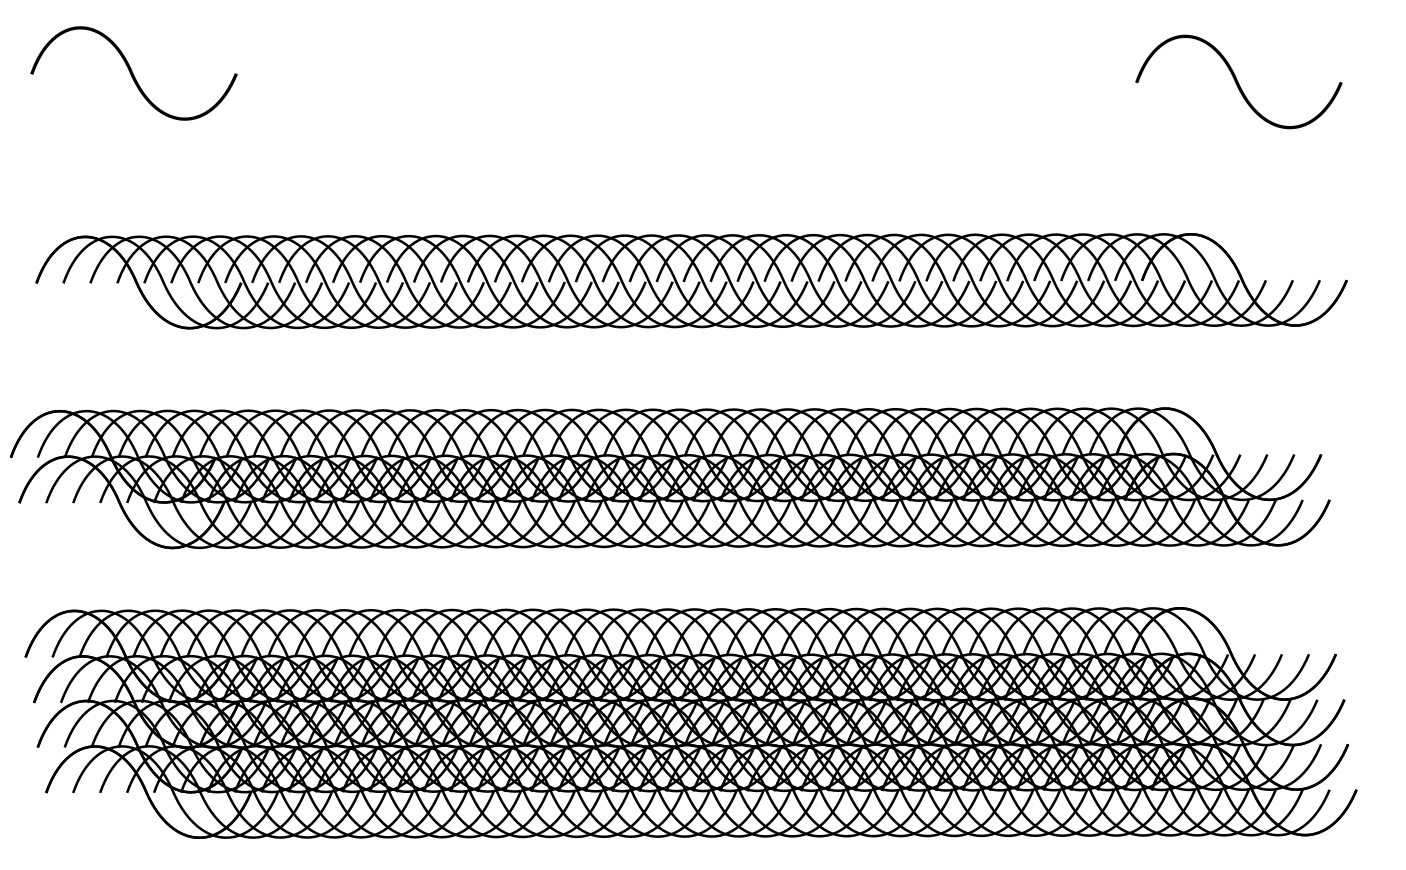
\includegraphics[width=1\linewidth]{1_pic.png}}
    \end{minipage}
\end{figure}
